% Options for packages loaded elsewhere
\PassOptionsToPackage{unicode}{hyperref}
\PassOptionsToPackage{hyphens}{url}
\PassOptionsToPackage{dvipsnames,svgnames,x11names}{xcolor}
%
\documentclass[
  letterpaper,
  abstract]{scrartcl}

\usepackage{amsmath,amssymb}
\usepackage{iftex}
\ifPDFTeX
  \usepackage[T1]{fontenc}
  \usepackage[utf8]{inputenc}
  \usepackage{textcomp} % provide euro and other symbols
\else % if luatex or xetex
  \usepackage{unicode-math}
  \defaultfontfeatures{Scale=MatchLowercase}
  \defaultfontfeatures[\rmfamily]{Ligatures=TeX,Scale=1}
\fi
\usepackage{lmodern}
\ifPDFTeX\else  
    % xetex/luatex font selection
\fi
% Use upquote if available, for straight quotes in verbatim environments
\IfFileExists{upquote.sty}{\usepackage{upquote}}{}
\IfFileExists{microtype.sty}{% use microtype if available
  \usepackage[]{microtype}
  \UseMicrotypeSet[protrusion]{basicmath} % disable protrusion for tt fonts
}{}
\makeatletter
% \@ifundefined{KOMAClassName}{% if non-KOMA class
  % \IfFileExists{parskip.sty}{%
  %   \usepackage{parskip}
  % }{% else
  %   % \setlength{\parindent}{pt}
  %   \setlength{\parskip}{6pt plus 2pt minus 1pt}}
% }{% if KOMA class
  % \KOMAoptions{parskip=half}}
\makeatother
\usepackage{xcolor}
\usepackage[margin=1.1in,letterpaper]{geometry}
\setlength{\emergencystretch}{3em} % prevent overfull lines
\setcounter{secnumdepth}{5}
% Make \paragraph and \subparagraph free-standing
\ifx\paragraph\undefined\else
  \let\oldparagraph\paragraph
  \renewcommand{\paragraph}[1]{\oldparagraph{#1}\mbox{}}
\fi
\ifx\subparagraph\undefined\else
  \let\oldsubparagraph\subparagraph
  \renewcommand{\subparagraph}[1]{\oldsubparagraph{#1}\mbox{}}
\fi


\providecommand{\tightlist}{%
  \setlength{\itemsep}{0pt}\setlength{\parskip}{0pt}}\usepackage{longtable,booktabs,array}
\usepackage{calc} % for calculating minipage widths
% Correct order of tables after \paragraph or \subparagraph
\usepackage{etoolbox}
\makeatletter
\patchcmd\longtable{\par}{\if@noskipsec\mbox{}\fi\par}{}{}
\makeatother
% Allow footnotes in longtable head/foot
\IfFileExists{footnotehyper.sty}{\usepackage{footnotehyper}}{\usepackage{footnote}}
\makesavenoteenv{longtable}
\usepackage{graphicx}
\makeatletter
\def\maxwidth{\ifdim\Gin@nat@width>\linewidth\linewidth\else\Gin@nat@width\fi}
\def\maxheight{\ifdim\Gin@nat@height>\textheight\textheight\else\Gin@nat@height\fi}
\makeatother
% Scale images if necessary, so that they will not overflow the page
% margins by default, and it is still possible to overwrite the defaults
% using explicit options in \includegraphics[width, height, ...]{}
\setkeys{Gin}{width=\maxwidth,height=\maxheight,keepaspectratio}
% Set default figure placement to htbp
\makeatletter
\def\fps@figure{htbp}
\makeatother

\KOMAoption{captions}{tableheading}
\makeatletter
\@ifpackageloaded{caption}{}{\usepackage{caption}}
\AtBeginDocument{%
\ifdefined\contentsname
  \renewcommand*\contentsname{Table of contents}
\else
  \newcommand\contentsname{Table of contents}
\fi
\ifdefined\listfigurename
  \renewcommand*\listfigurename{List of Figures}
\else
  \newcommand\listfigurename{List of Figures}
\fi
\ifdefined\listtablename
  \renewcommand*\listtablename{List of Tables}
\else
  \newcommand\listtablename{List of Tables}
\fi
\ifdefined\figurename
  \renewcommand*\figurename{Figure}
\else
  \newcommand\figurename{Figure}
\fi
\ifdefined\tablename
  \renewcommand*\tablename{Table}
\else
  \newcommand\tablename{Table}
\fi
}
\@ifpackageloaded{float}{}{\usepackage{float}}
\floatstyle{ruled}
\@ifundefined{c@chapter}{\newfloat{codelisting}{h}{lop}}{\newfloat{codelisting}{h}{lop}[chapter]}
\floatname{codelisting}{Listing}
\newcommand*\listoflistings{\listof{codelisting}{List of Listings}}
\makeatother
\makeatletter
\makeatother
\makeatletter
\@ifpackageloaded{caption}{}{\usepackage{caption}}
\@ifpackageloaded{subcaption}{}{\usepackage{subcaption}}
\makeatother
\ifLuaTeX
  \usepackage{selnolig}  % disable illegal ligatures
\fi
\usepackage[sorting=none, style=numeric-comp]{biblatex}
\addbibresource{../library.bib}
\usepackage{bookmark}
\usepackage{xcolor}
\definecolor{myorange}{RGB}{240, 96, 0}
\newcommand{\mt}[1]{{\textcolor{myorange} {({\tiny MT:} #1)}}}
\newcommand\numberthis{\addtocounter{equation}{1}\tag{\theequation}}

\IfFileExists{xurl.sty}{\usepackage{xurl}}{} % add URL line breaks if available
\urlstyle{same} % disable monospaced font for URLs
\hypersetup{
  pdftitle={Predicting the effect of candidate interventions for mitigating disease spread in asymmetric mixing metapopulations},
  colorlinks=true,
  linkcolor={blue},
  filecolor={Maroon},
  citecolor={Blue},
  urlcolor={Blue},
  pdfcreator={LaTeX via pandoc}}

\title{Predicting the effect of candidate interventions for mitigating
disease spread in asymmetric-mixing metapopulations}
\author{Matthew Adam Turner}
\date{\today}

\begin{document}
\maketitle
\begin{abstract}
\noindent hello
\end{abstract}

\renewcommand*\contentsname{Table of contents}
{
\hypersetup{linkcolor=}
\setcounter{tocdepth}{3}
\tableofcontents
}
\section{Introduction}\label{introduction}

To equitably prepare for pandemics in our uncertain world we
need to predict the effect of candidate interventions to mitigate novel spillover
disease and novel variants of existing disease
\autocite{Rodo2021,Adashi2022}. The global COVID-19 pandemic highlighted
the current lack of outcome equality, where a country's inequality
(measured by the Gini index) predicted higher burden of COVID-19
infections \autocite{Su2022}. Here we contribute to this program of more
equitable pandemic preparedness by developing a compartmental
behavioral-epidemiological metapopulation model with an immediate application:
disease transmission between a Brazilian city, Dourados, in the state of 
Mato Grosso do Sul, and the
neighboring Dourados Indigenous Reserve \autocite{DeOliveira2023}.
COVID-19 burden was felt disproportionately by Indigenous peoples throughout
Brazil \autocite{Simionatto2020}, but the burden may have been even more 
inequitable in the
Dourados Reserve due to its immediate proximity to the city of Dourados. Nearly
all residents of the reserve live in domiciles in one of two villages in
the Reserve, Jaguapiru and Bororó. Jaguapiru is closer overall to the
city of Dourados, sharing a much longer border with the city limits than
Bororó (Figure \ref{fig:Map}). Indigenous peoples on the reserve are predominantly
one of two ethnicities, Guarani and Terena. 
% Anecdotally, Terena are
% known for being better educated with somewhat more robust physicality
% and, perhaps, better resistance to disease. 
% Anecdotally Terena may travel to the city more frequently for trade and other purposes,
% however De Olivera and colleagues 
De Oliveira and co-authors hypothesized that COVID-19 variant diffusion
from Dourados City into the Dourados Reserve is driven by young
Indigenous men traveling between the reserve and the city of Dourados
for economic reasons. This is a reasonable starting hypothesis given available
data, but it points to potentially richer, more explanatory mechanisms and 
a more detailed set of hypotheses. Understanding transmission in the Reserve, and
evaluating possible interventions based on this understanding, could mitigate
the next pandemic that affects the Dourados Reserve, and lessons learned here could
transfer to pandemic preparedness planning in other contexts.

Despite some evidence to support the hypothesis that young male
Indigenous mobility can explain transmission into the reserve, there are
many complicating factors that make it difficult to evaluate this
hypothesis directly without adding some additional qualifications. 
There
may be other social factors that may be necessary for the time series
observations of De Oliveira and co-authors. 
Furthermore, there may be
less significant factors driving transmission in this model that may be
of greater importance in future outbreaks of different diseases than
SARS-CoV-2 in the reserve. 
Therefore, here we expand the scope of the
hypothesis to include hypotheses about how social groups, namely village
residency and Indigenous ethnic group, affect transmission in the
reserve and explain observed outbreaks of variants B.1.1 and Zeta in the
Reserve. To evaluate the hypotheses, presented in the next paragraph, we
develop a mechanistic model of epidemiological transmission with
asymmetric social mixing that evaluates how best to model group
structure in the Reserve. In turn, this model is used to evaluate
potential economic interventions that target aid to different groups to
reduce infections in the reserve.

\vspace{0.5em}
\begin{center}
{[ FIGURE \ref{fig:Map} ABOUT HERE ]} \\
\end{center}

\vspace{0.5em}
\begin{center}
{[ FIGURE \ref{fig:DeOliveiraSeries} ABOUT HERE ]} \\
\end{center}


\begin{itemize}
\item
  De Oliveira and colleagues tracked the spread of different SARS-CoV-2
  variants by village and by variant.
\item
  The goal of our model is two-fold. First, to identify parameters that
  could re-create the time series plots in Figure 1.
\item
  Second, we aim to use a parameterized model to understand how
  different intervention strategies could reduce infections among
  Reserve residents. For example, perhaps since Terena are suspected to
  travel to the
\item
  While we know a lot about transmission in the reserve, and the work of
  de Oliveira and colleagues advanced our understanding of transmission
  in the Reserve, we do not have reliable estimates of exactly how many
  cases there were per ethnicity and village. We also have only
  word-of-mouth information about the frequency of travel to the city
  for each ethnicity and location. Our model motivates the need for a
  more thorough understanding of behavior and epidemiological parameters
  in the Dourados Indigenous Reserve, and points the way towards future
  research in other Indigenous communities, and more complex situations.
  Here we only consider Indigenous mobility, but many people from the
  city travel to the reserve for commerce as well.
\end{itemize}

\section{Model}\label{sec:model}

To understand and predict how different candidate economic interventions could
reduce transmission in the Dourados Reserve, we develop a mechanistic model of
transmission in the Reserve implemented as a set of compartmental
susceptible-infected-recovered system (SIR) of differential equations.  There
are six compartments in the differential equations, one $S_g$, $I_g$, and $R_g$ for
each group, $g$.  We evaluate different interventions by varying the reduction in
Indigenous travel between the Dourados reserve and the city, which in the real
world would be achieved by economic aid that reduces the need for Indigenous
travel to the city. First we test the effect of global reduction in travel on
infections in the Reserve, where aid is distributed equally across all possible
groupings. Second, we test different strategies for distributing aid to
different groups to understand which, if any, are more effective than equal aid
distribution. Finally, we test infectin prevention under both global and
group-specific intervention strategies for a stylized version of the Zeta
variant that allows probabilistically for re-infection. Although the model is
focused on COVID-19 transmission in the Dourados Indigenous Reserve, the
model is abstract. What we learn in our analyses could therefore transfer to
other diseases in the Reserve or other socio-epidemiological contexts.


\subsection{Model dynamics and formalism}
\label{sub:modelDynamics}

Our model represents interactions within and between Dourados Indigenous 
Reserve groups, and with members of the city of Dourados 
(Figure~\ref{fig:ModelSketch}). To represent
interactions between groups we define two possible groupings, by village
(Figure~\ref{fig:ModelSketch}, Model 1) and by ethnicity
(Figure~\ref{fig:ModelSketch}, Model 2). The within-group contact rate 
is $c_{gg}$ for focal group $g$. The contact rate between the focal group and
its outgroup, $g'$, is $c_{gg'}$. If in Model 2 the focal group is Terena, then
the within-group contact rate is $c_{TT}$ and the between-group contact rate,
representing how frequently Terena interact with Guarani is $c_{TG}$, Each of these groupings can be further
subdivided by the alternative Model grouping, represented in 
Figure~\ref{fig:ModelSketch} by the inset pie chart diagrams in each group's
circle. Reserve resident mobility is represented by a contact-infection rate,
$\gamma_g$, which represents how frequently a susceptible member of group $g$
brings an infection into the Reserve. The exact compartments, $S$, $I$, and $R$
for the city population are ignored.

\vspace{0.5em}
\begin{center}
{[ FIGURE \ref{fig:ModelSketch} ABOUT HERE ]} \\
\end{center}

This contact structure, combined with a global transmission rate $\tau$,
recovery rate, $\rho$, and re-susceptibility rate, $r$, results in a system of
six differential equations for each of the six compartments
(Equation~\ref{eq:DiffEqs}). $\tau$ and $\rho$ will be set to reasonable values
for main analyses, but varied for sensitivity analyses.  \mt{Q: What constitutes
a ``reasonable value'' here? Values Aja used were for ABM---what about for a
diffeq model like this?}. To model increased re-infections observed with the
Zeta variant, we also include a term $r R_g$ that is positive in the
$\frac{dS_g}{dt}$ equation and negative in the $\frac{dR_g}{dt}$ term to
transfer recovered individuals from the recovered compartment for group $g$ to
the susceptible compartment for that group. If $r=0$, then there will be no
re-infections. Otherwise there may be re-infections, which could have complex
interactions with interaction structure.

\begin{align*}
  \frac{dS_g}{dt} &= -m_{gg'} \tau S_g + r R_g   \\
  \frac{dI_g}{dt} &=  m_{gg'} \tau S_g - \rho I_g \\
  \frac{dR_g}{dt} &= \rho I_g - r R_g,\quad\text{ where } \\[1em]
          m_{gg'} &= \left(c_{gg'} I_g + c_{g'g}I_{g'} + \gamma_g \right)
    \numberthis \label{eq:DiffEqs}
\end{align*}
\noindent


\vspace{0.5em}
\begin{center}
{[ TABLE \ref{tab:ModelVariables} ABOUT HERE ]} \\
\end{center}



\subsection{Computational analysis}

We evaluate hypothetical interventions to limit the spread of
infection in the Reserve by simulating these interventions using the formal
system explained above. Our main outcome variable is the mean reduction 
in simulated COVID-19 incidence among group $g$ as a fraction of the no-intervention
cumulative cases, defined at the group level as
\begin{equation}
  \langle \Delta I_g \rangle = \left\langle \frac{I^\mathrm{Tot}_g(\text{no intervention}) -
    I^\mathrm{Tot}_g(\text{intervention } i)}{I^\mathrm{Tot}_g(\text{no
  intervention})} \right\rangle.
  \label{eq:DeltaI_byGroup}
\end{equation}
\noindent
The mean total expected reduction of cumulative cases is 
\begin{equation}
  \langle \Delta I^\mathrm{Tot} \rangle = \left \langle \sum_g \Delta I_g \right \rangle = \sum_g \left \langle \Delta I_g \right \rangle 
  \label{eq:DeltaI}
\end{equation}
\noindent
by linearity of expectations.
In the case of deterministic differential equations, these expectations are just the
values themselves.  We can define A preliminary step is to find parameterizations
that reproduce the observed outbreaks of B.1.1 and Zeta within the Reserve to obtain
a baseline estimate of infection size $I(\text{no intervention})$.  To this end we
hypothesize that re-infections could have driven the observed greater spread of the
Zeta strain, though it could also be due to the holiday season around the end of
2020 and beginning of 2021. 

Interventions center around reducing the mobility of Indigenous people between
Dourados city and Reserve; the total change in mobility, denoted $\Delta
\gamma$, is the total reduction of the parameter $\gamma_g$ across all 
groups, i.e., 
\begin{equation}
  \Delta \gamma = \sum_g \Delta \gamma_g.
  \label{eq:DeltaGamma}
\end{equation}
\noindent
Different interventions allocate $\Delta \gamma$ (Equation~\ref{eq:DeltaGamma})
in different ways to hypothetically result in different case reductions for each
group and overall (Equation~\ref{eq:DeltaI_byGroup} and Equation~\ref{eq:DeltaI},
respectfully; see Table~\ref{tab:AnalysisVariables} for a summary of these analysis
variables).
One strategy we test is the \emph{Equal} strategy, where all $\gamma_g$ are
equal. Another named strategy is the \emph{80-20} strategy, where the
reduction in mobility in group $g$ is 80\% of the total, and reduction in
group $g'$ mobility is 20\% of the total, i.e., $\Delta\gamma_g / \Delta\gamma =
0.8$ and $\Delta\gamma_{g'} / \Delta\gamma = 0.2$. To create alternative
strategies, both the total reduction and the ratio of group-level reduction to 
total reduction can be changed. In addition to total case reduction, we 
measure relative group-level case reduction, $\Delta I_g$, 
for each considered strategy to understand whether case reduction is equitable
between villages and ethnicities under different strategies. 
We finally evaluate the hypothesis that interventions that may be effective for
strains with no re-infection (like B.1.1) will not be equally effective for
strains with re-infection (like Zeta), and vice-versa. 
% This will highlight the importance of accounting for social and
% epidemiological context, alike, in predicting the effectiveness of mitigation
% strategies for pandemic preparedness.


\section{Analysis (Sketch)}\label{analysis-sketch}




\vspace{0.5em}
\begin{center}
{[ FIGURE \ref{fig:ByGroupReduction_GlobalStrategy} ABOUT HERE ]} \\
\end{center}

% \vspace{0.5em}
% \begin{center}
% {[ FIGURE \ref{fig:ByReinfectionByStrategy} ABOUT HERE ]} \\
% \end{center}

\vspace{0.5em}
\begin{center}
{[ FIGURE \ref{fig:ByReinfectionByStrategy} ABOUT HERE ]} \\
\end{center}


\section{Discussion}\label{discussion}


\begin{itemize}
  \item 
    Application to other problematic diseases in the Reserve, e.g., TB, STDs,\ldots 
  \item
    The data is not necessarily representative and we had to use educated guesses
    for mixing parameters.
  \item
    Have not yet considered more complex epidemiological and behavioral
    dynamics. For example, group structure can affect the coupled contagion of
    disease and behaviors that could encourage or impede the spread of
    disease~\autocite{SmaldinoJones2021}. Our compartmental model
    incorporated group structure and contact rate heterogeneity, but finer
    details of the social network structure can induce complex
    epidemiological dynamics~\autocite{Arthur2017}. In the case of Dourados
    and possibly other Indenous communities is the tendency for several
    generations of families to live in close proximinty to one another,
    often communally with other families as well, making social isolation
    culturally unpalatable and, consequentially, unfeasible. Adaptation to
    evolving, uncertain epidemiological social and environmental contexts is
    one further factor that can complicate epidemiological
    dynamics~\autocite{Arthur2021} and willingness to learn beneficial public
    health behaviors from others~\autocite{Turner2023a}.
\end{itemize}


\printbibliography[title=References]


\clearpage

\section{Tables}


\begin{table}[h]
  \centering
  \caption{\textbf{Model variables, description and values taken.} The
  compartmental model described in Equation~\ref{eq:DiffEqs} includes several
social mixing, behavioral, and epidemiological variables described here.}
  \label{tab:ModelVariables}
  \begin{tabular}{rlp{1.3in}} 
    \toprule
    variable & description & values \\ 
    \midrule 
    $S_g,I_g,R_g$ & Susceptible, infected, recovered compartments by group & $[0.0,1.0]$ \\
    $c_{gg'},c_{g'g}$ & Asymmetric inter-group contact rates & $[0.0,1.0]$ \\
    $\gamma_g$ & Group-level incidence-contact rate with city residents &
      $\{0.0,0.1,\ldots,0.4\}$ \\
    $\rho$ & Global recovery rate & $[0.0,1.0]$ \\
    $\tau$ & Global ransmission rate & $[0.0,1.0]$ \\
    $r$    & Re-susceptible probability, non-zero only for Zeta & $0.0,0.5$ \\
    $g,g'$ & Reference group ($g$) and out-group $g'$ & Terena, Guarani; Bororó, Jaguapiru \\
    \bottomrule
  \end{tabular} 
\end{table}



\begin{table}[h]
  \centering
  \caption{\textbf{Independent and dependent analysis variables.} Reducing
  mobility to the city (first row) hypothetically increases the reduction in
cumulative cases in the Reserve (second row).}
  \label{tab:AnalysisVariables}
  \begin{tabular}{rp{3.0in}l} 
    \toprule
    variable & description & values \\
    \midrule 
    $\Delta \gamma$ and $\Delta \gamma_g$ & Total city mobility reduction and 
      group-level mobility reduction & $0.0,0.2,\ldots,0.8$ \\
      $\langle \Delta I^\mathrm{Tot} \rangle$ and $\langle \Delta I^\mathrm{Tot}_g
      \rangle$  & Parameter-set ensemble averages of total and group-level
      cumulative incidence reduction & [0.0, 1.0] \\
    \bottomrule
  \end{tabular} 
\end{table}



\section{Figures}

\begin{figure}[H]

\centering
\caption{\textbf{Map of Dourados Indigenous Reserve villages.} Bororó is light
blue, Jaguapiru cyan, and the city of Dourados dark blue. Note
Jaguapiru shares a much longer boundary with the reserve than Dourados,
which facilitates mobility in and out of the reserve for both Reserve
and city residents. Maps combined from Cavalcante (2019) for the underlying
topographic map and Schnaufer et al.~(2023) for the villages, city, and 
sample collection points (clinics) layer.}
\label{fig:Map}
\vspace{0.3em}
{\includegraphics[width=0.8\textwidth,height=\textheight]{Figures/ReserveMap.pdf}}
\end{figure}%%


\begin{figure}[H]
\caption{Time series of COVID-19 spread through the Dourados Indigenous
Reserve, with significant events highlighted. The first B.1.1 variant
cases were introduced by the Guarani ethnicity (1), followed about one
month later by a rapid rise in cases in Jaguapiru among the Terena
ethnicity (2); several months later a rapid rise in Bororó was caused by
a rapid rise among Guarani (3). Zeta was introduced at the end of 2020
(4), with a rapid rise around the holiday season especially in Jaguapiru
among Guarani (5); later in February cases rose in Bororó among the
Terena (6).}
\label{fig:DeOliveiraSeries}
\vspace{0.3em}
{\centering 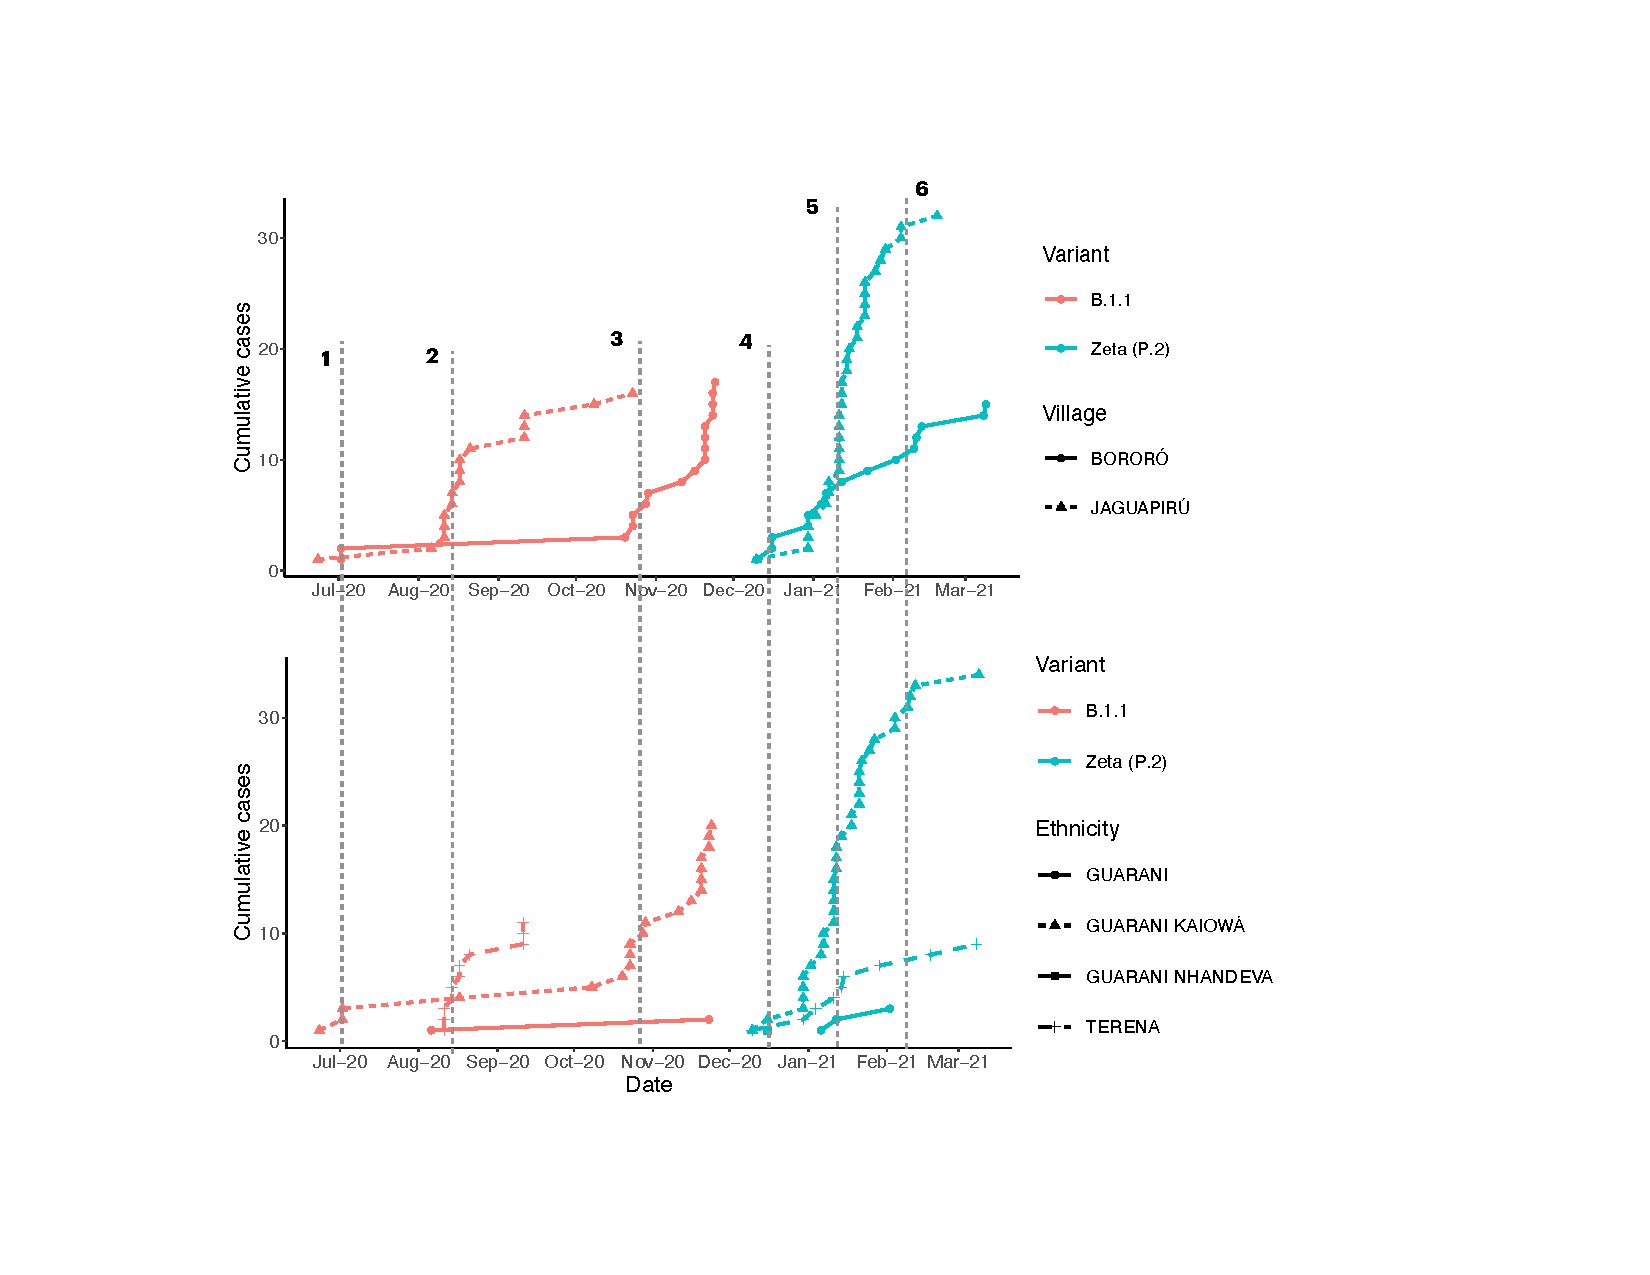
\includegraphics[width=0.8\textwidth,height=\textheight]{Figures/Time Series.pdf}

}
\end{figure}%



\begin{figure}[H]

\caption{
  We can model the relevant groups for mixing as either village
residence or ethnicity. Mixing, and mobility parameters
would be set accordingly. Mixing is asymmetric, with $c_{gg}$ representing the
contact rate within group $g$, and each $c_{gg'}$ representing
the contact rate at which a member of group $g$ encounters a member of the
outgroup $g'$, e.g., $c_{GT}$ is the contact rate at which Guarani encounter
members of the Terena. The $\gamma_g$ parameters would be reduced through
economic aid to group $g$ for them to remain on the Reserve during
outbreaks. \mt{Looks like some labels are cut off; will fix in later draft.}}
\label{fig:ModelSketch}
\vspace{0.3em}
{\centering 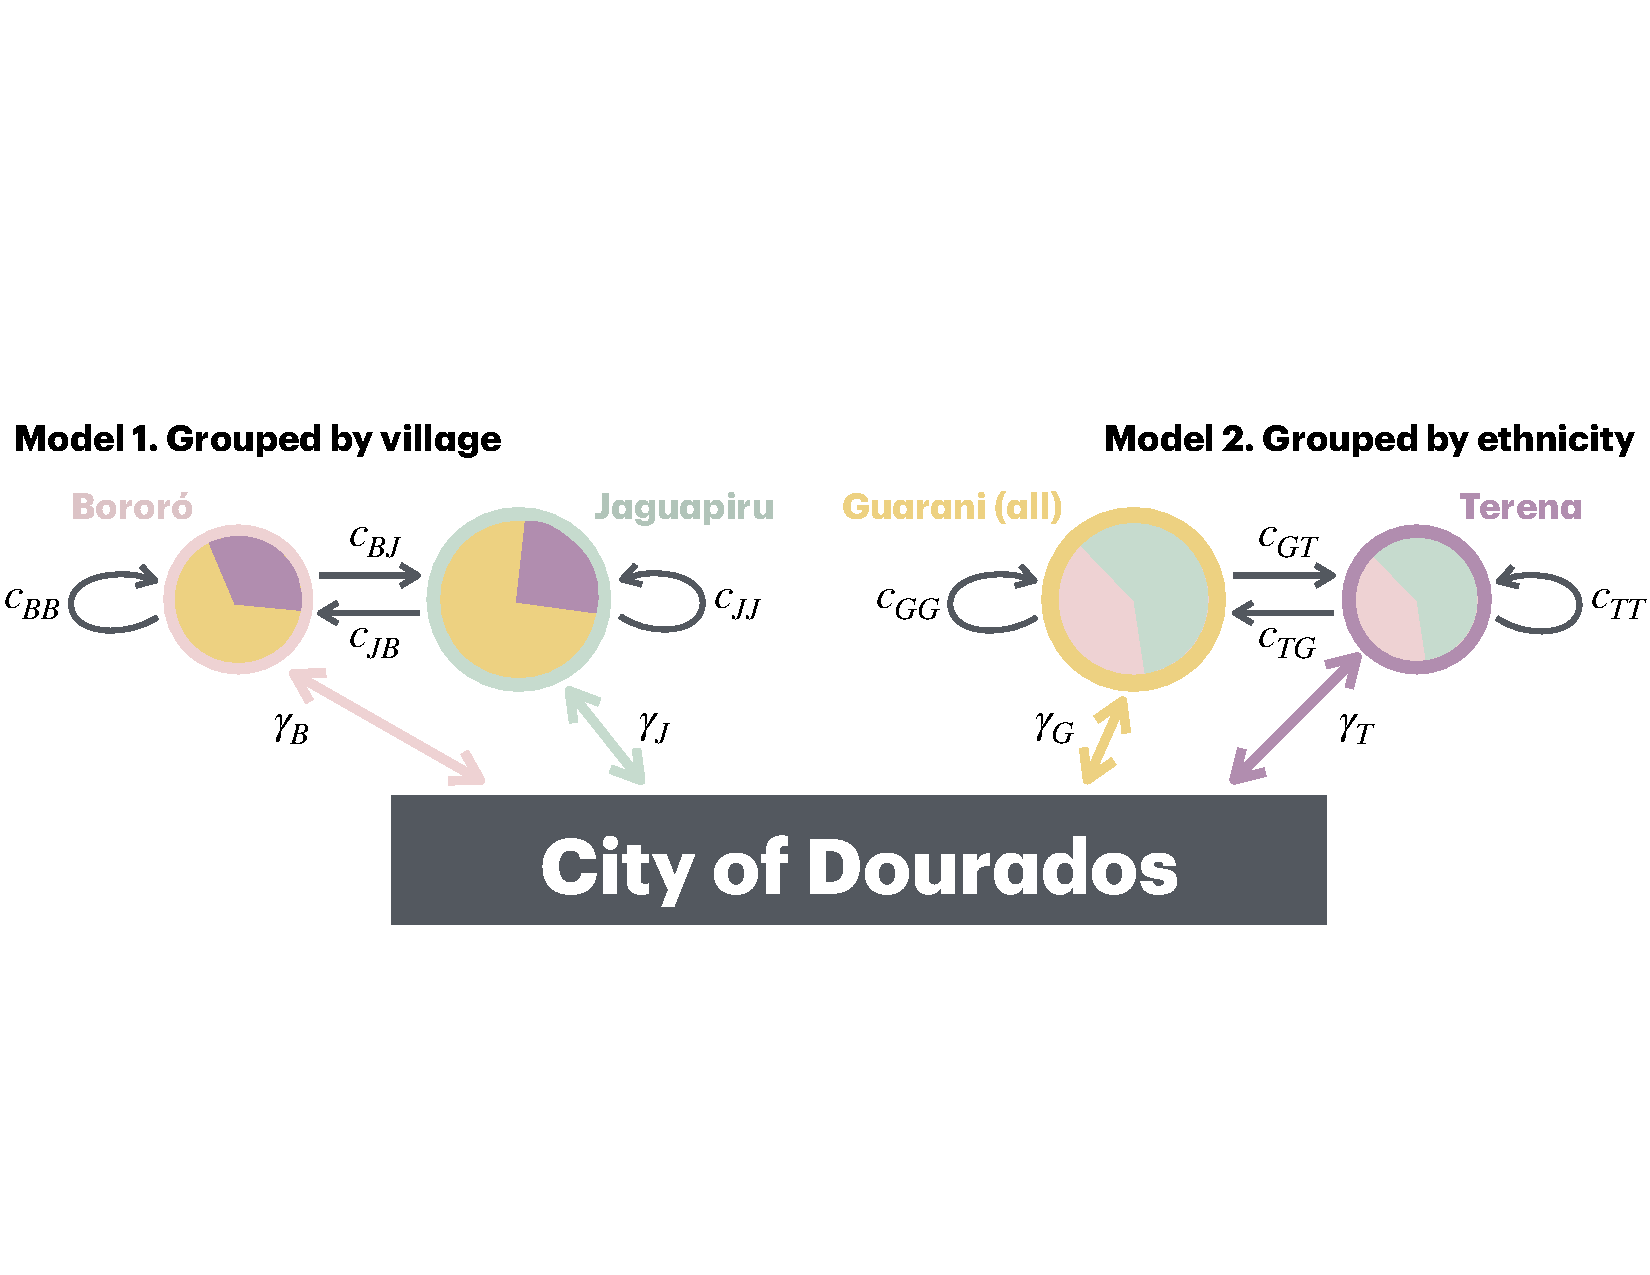
\includegraphics{Figures/ModelSketch.pdf}

}
\end{figure}%





% \begin{figure}[H]

% \caption{We hypothesize that overall reduction in disease incidence ($\Delta I$, y-axis)  depends on 
% strategy to distribute the total aid to reduce travel between Dourados Reserve and city ($\Delta \gamma$, x-axis).}
% \label{fig:ByGroupReduction_GlobalStrategy}
% \vspace{0.3em}
% {\centering 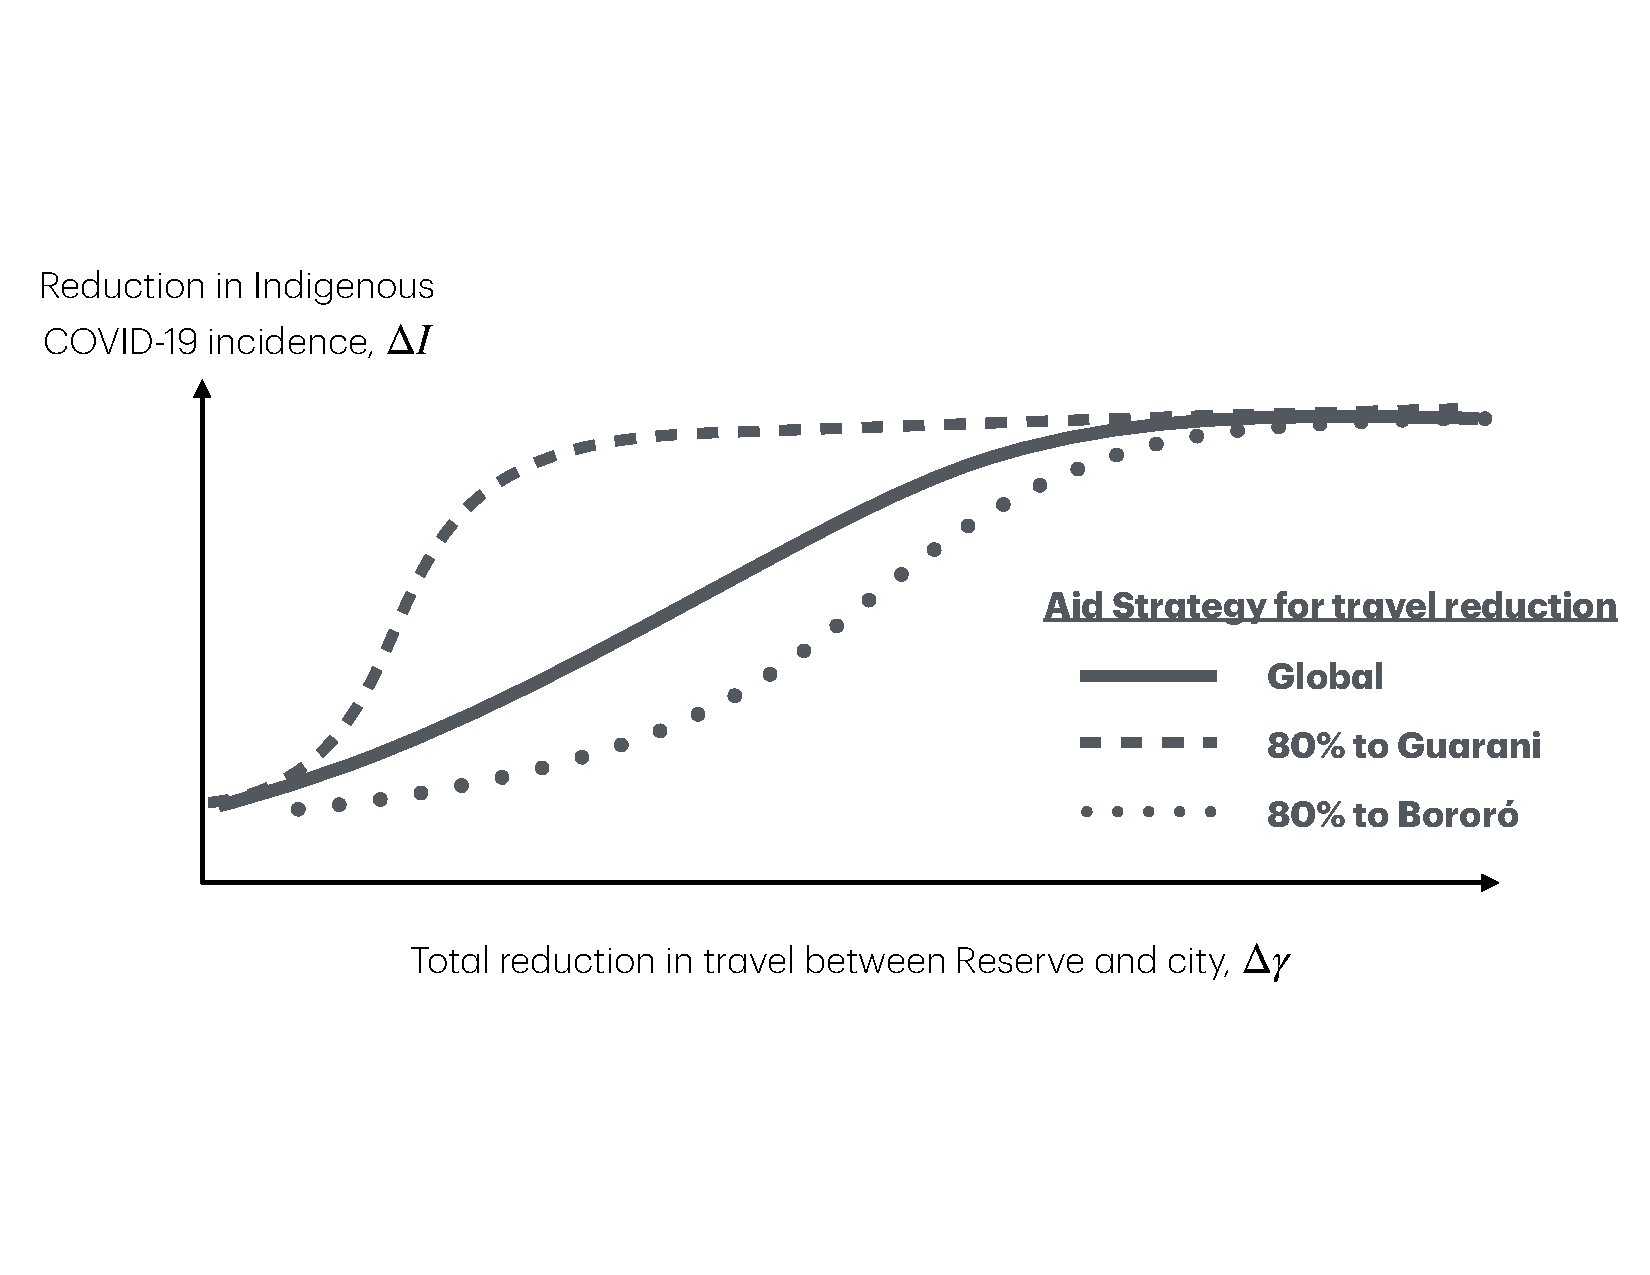
\includegraphics[width=0.95\textwidth,height=\textheight]{Figures/ResultsSketch_ByStrategy.pdf}

% }
% \end{figure}


\begin{figure}[H]

\caption{Disease reduction ($\Delta I$, y-axis) depends on the possibility of
  re-infection and the
distribution strategy to reduce travel between Dourados Reserve and city ($\Delta \gamma$, x-axis).}
\label{fig:ByReinfectionByStrategy}
\vspace{0.3em}
{\centering
  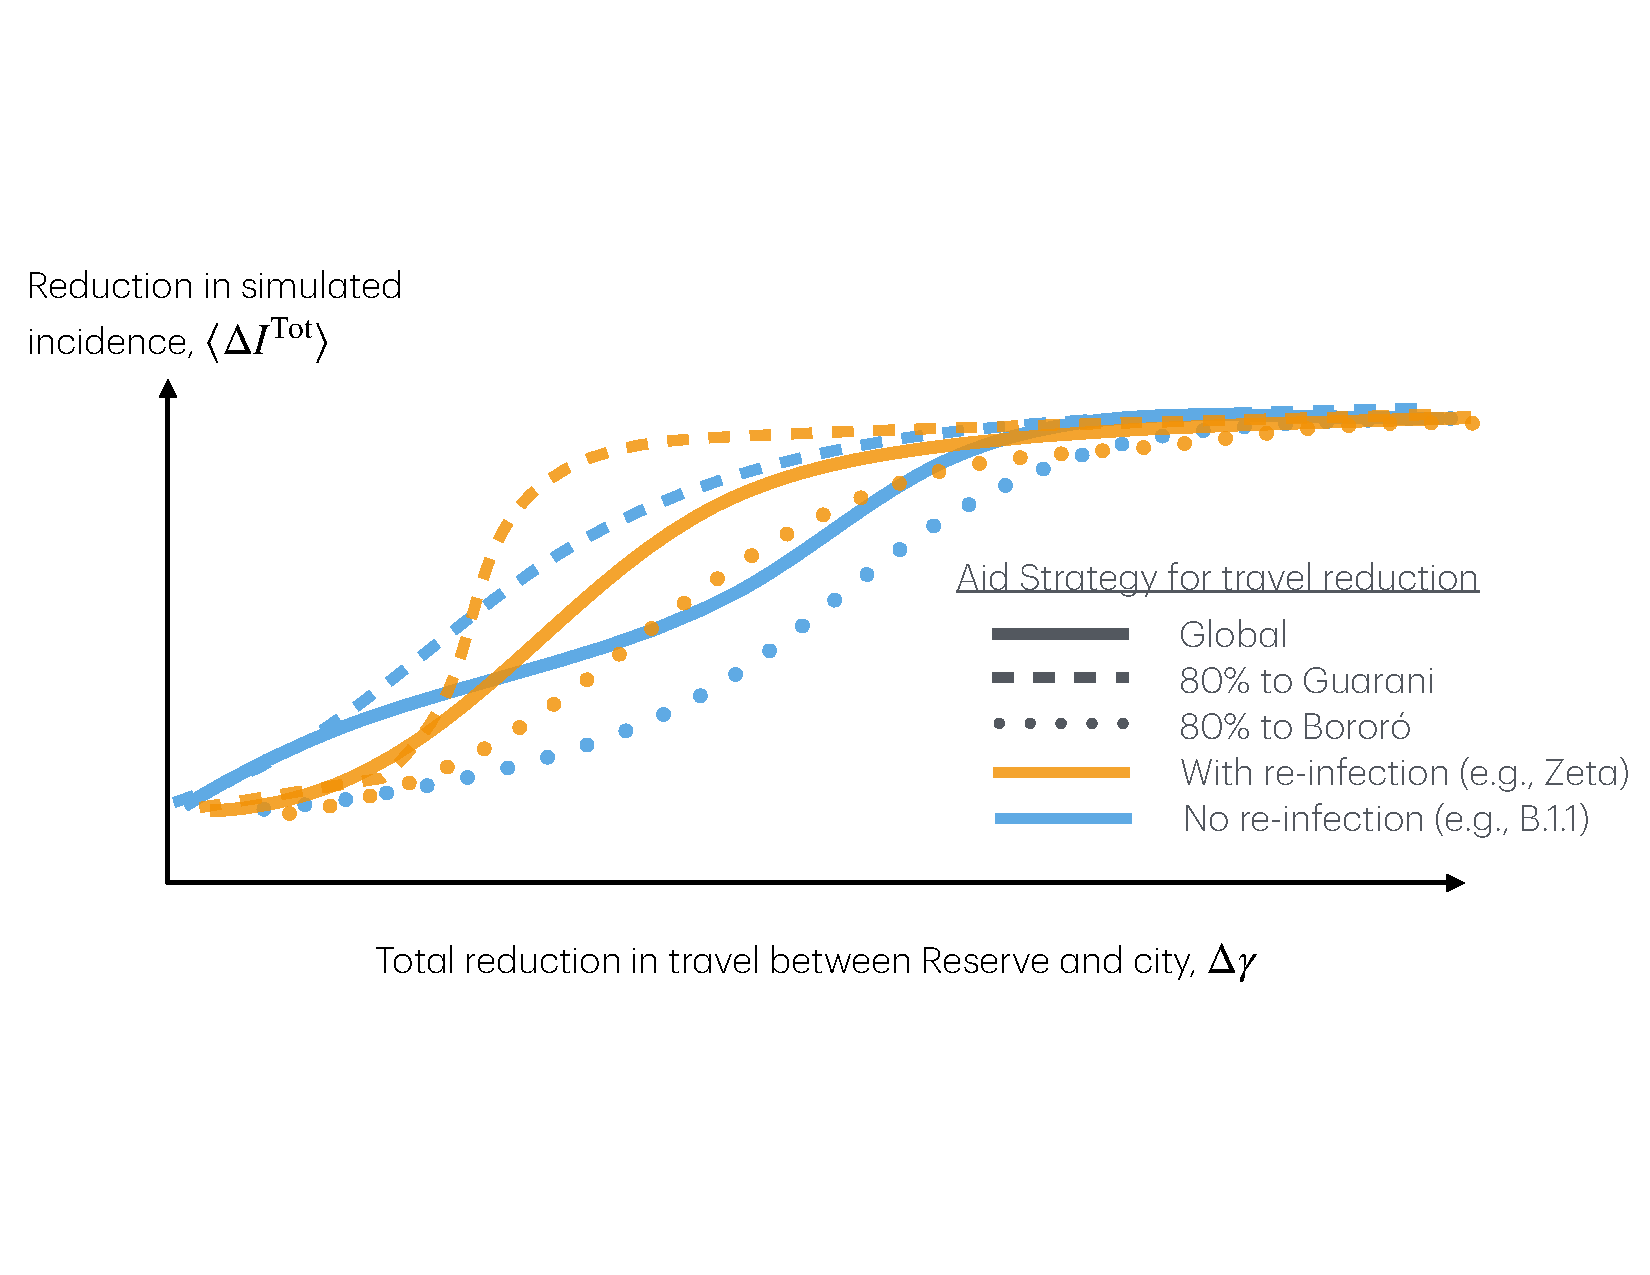
\includegraphics[width=0.95\textwidth,height=\textheight]{Figures/ResultsSketch_ByReinfectionByStrategy.pdf}

}


\end{figure}%

\begin{figure}[H]

\caption{Global reduction in travel to and from the city could have
Infection reduction ($\Delta I$, y-axis) for different groups could be
different as global reduction in travel to and from the city decreases
($\Delta \gamma$, x-axis).}
\label{fig:ByGroupReduction_GlobalStrategy}
\vspace{0.3em}
{\centering 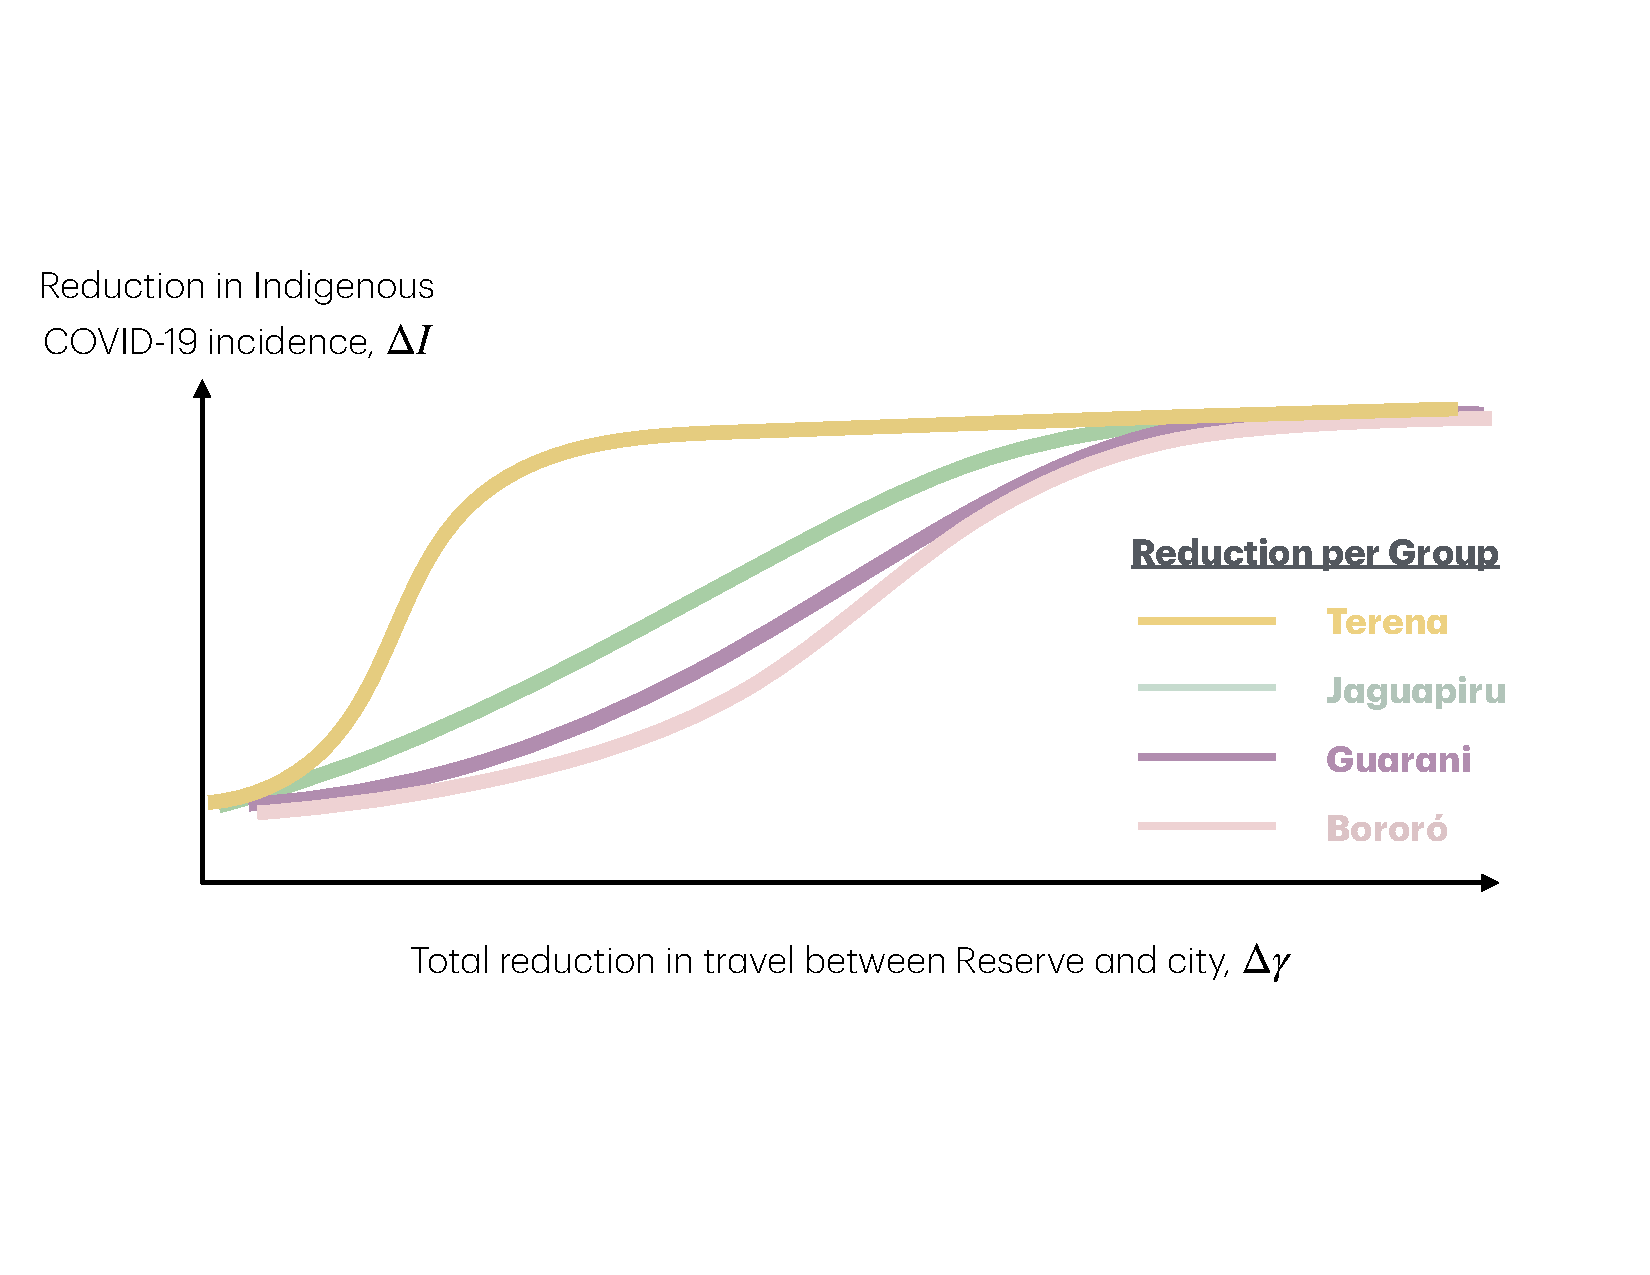
\includegraphics[width=0.95\textwidth,height=\textheight]{Figures/ResultsSketch_ReductionByGroup.pdf}

}

\end{figure}%

\end{document}
